%\documentclass[aspectratio=10]{beamer} %For normal presentation (comment otherwise)
\documentclass[aspectratio=169]{beamer} %for widescreen prestentation
\usetheme{default}%{Singapore}
\usefonttheme{serif}
\usepackage{ulem}
\usecolortheme{default}%albatross, crane, beetle, dove, fly, seagull, wolverine e beaver.
\setbeamertemplate{frametitle}[default][center]
%%%%%%%%%%%%%%%%%%%%%%%%%%%%%%%%%%%%%%%%%%%%%%%%%%%%%%%%%%%%%%%%%%%%%%%%%%%%%%%%%%%%%%%%%%%%%%%
%%%%%%%%%%%%%%%%%%%%%%%%%%%%%%%%%%%%%%EXTRA PACTAGES%%%%%%%%%%%%%%%%%%%%%%%%%%%%%%%%%%%%%%%%%%%
\usepackage[utf8]{inputenc}
\usepackage[T1]{fontenc}
\usepackage[scaled]{helvet}
\renewcommand*\familydefault{\sfdefault}
\usepackage[portuguese, english]{babel}
\usepackage[round]{natbib}
\usepackage{hyperref} 
\usepackage{tcolorbox}
\usepackage{graphicx} % Required for including images
\usepackage{graphics}
%\usepackage[dvips]{graphicx} 
\graphicspath{{images/}} % Location of the graphics files
\usepackage{booktabs} % Top and bottom rules for table
\usepackage[font=small,labelfont=bf]{caption}%specifies captions on tables and figures
\usepackage{amsfonts, amsmath, amsthm, amssymb} % For math fonts, symbols and environments
\usepackage{wrapfig} % Allows wrapping text around tables and figures
\usepackage{makeidx}
\usepackage{epstopdf}%adiciona imagens em formato eps no pdf.
\usepackage{subfigure}%cria ambientes de multifiguras
\usepackage{float}%coloca as figuras exatamente aonde você quer
\usepackage{times}
\usepackage{tikz}%pacote para fazer fluxogramas
\usepackage{epsfig}
\usepackage{graphicx}
\usepackage{epstopdf} %converting to PDF
\usepackage{verbatim}%
\usepackage{multicol}
\usepackage{xcolor}
\usepackage[makeroom]{cancel}
\usepackage[framemethod=tikz]{mdframed}
\usepackage{hyperref} 
\usepackage{smartdiagram}
\usepackage{amssymb}
\usepackage{etoolbox}
\usepackage{tikz}
\usetikzlibrary{mindmap}
\usepackage{metalogo}
%\smartdiagramset{uniform color list=gray!60!black for 6 items,
%back arrow disabled=false}
\usepackage{booktabs} % Top and bottom rules for table
\usepackage[font=small,labelfont=bf]{caption} % Required for specifying captions to 

%%%%%%%%%%%%%%%%%%%%%%%%%%%%%%%%%%%%%%%%%%%%%%%%%%%%%%%%%%%%%%%%%%%%%%%%%%%%%%%%%%%%%%%%%%%%%
%%%%%%%%%%%%%%%%%%%%%%%%%%%%%%%%%%%%% PREAMBLE %%%%%%%%%%%%%%%%%%%%%%%%%%%%%%%%%%%%%%%%%%%%%%%%
%\subtitle{}
\author[Victor Carreira]{} 
\title{A inteligência artificial é inteligente?}
\subtitle{Hunger of Science}
\institute{LOOP}
\date{Setembro de 2024}
\subject{Grupo LOOP}
%\setbeamertemplate{footline}[frame number]
%\setbeamercovered{transparent}
\setbeamertemplate{navigation symbols}{}
% Tela cheia
\hypersetup{pdfpagemode=FullScreen}
\usepackage{ragged2e}
%\justifying
%\addtobeamertemplate{headline}{}
\usepackage{tikz}
\usetikzlibrary{shapes.geometric, arrows}

% Criar um novo comando para destacar o primeiro item
\patchcmd{\sectioninToC}{\inserttocsection}{\ifnumequal{\inserttocsectionnumber}{1}{\textbf{\inserttocsection}}{\inserttocsection}}{}{}


%%%%%%%%%%%%%%%%%%%%%%%%%%%%%%%%%%%%%%%%%%%%%% PRESENTATION %%%%%%%%%%%%%%%%%%%%%%%%%%%%%%%%%%%%%%%%%%%%%%%
\begin{document}


\bgroup
\makeatletter
\setbeamertemplate{footline}
\makeatother
%\maketitle
\egroup
\scriptsize 
\addtobeamertemplate{navigation symbols}{}{\hskip6pt\raisebox{2pt}{\color{blue}\insertframenumber}}
\setcounter{framenumber}{0}
%\AtBeginSection[]


%%% Preambulo

%%% capa
{
\usebackgroundtemplate{
\centering
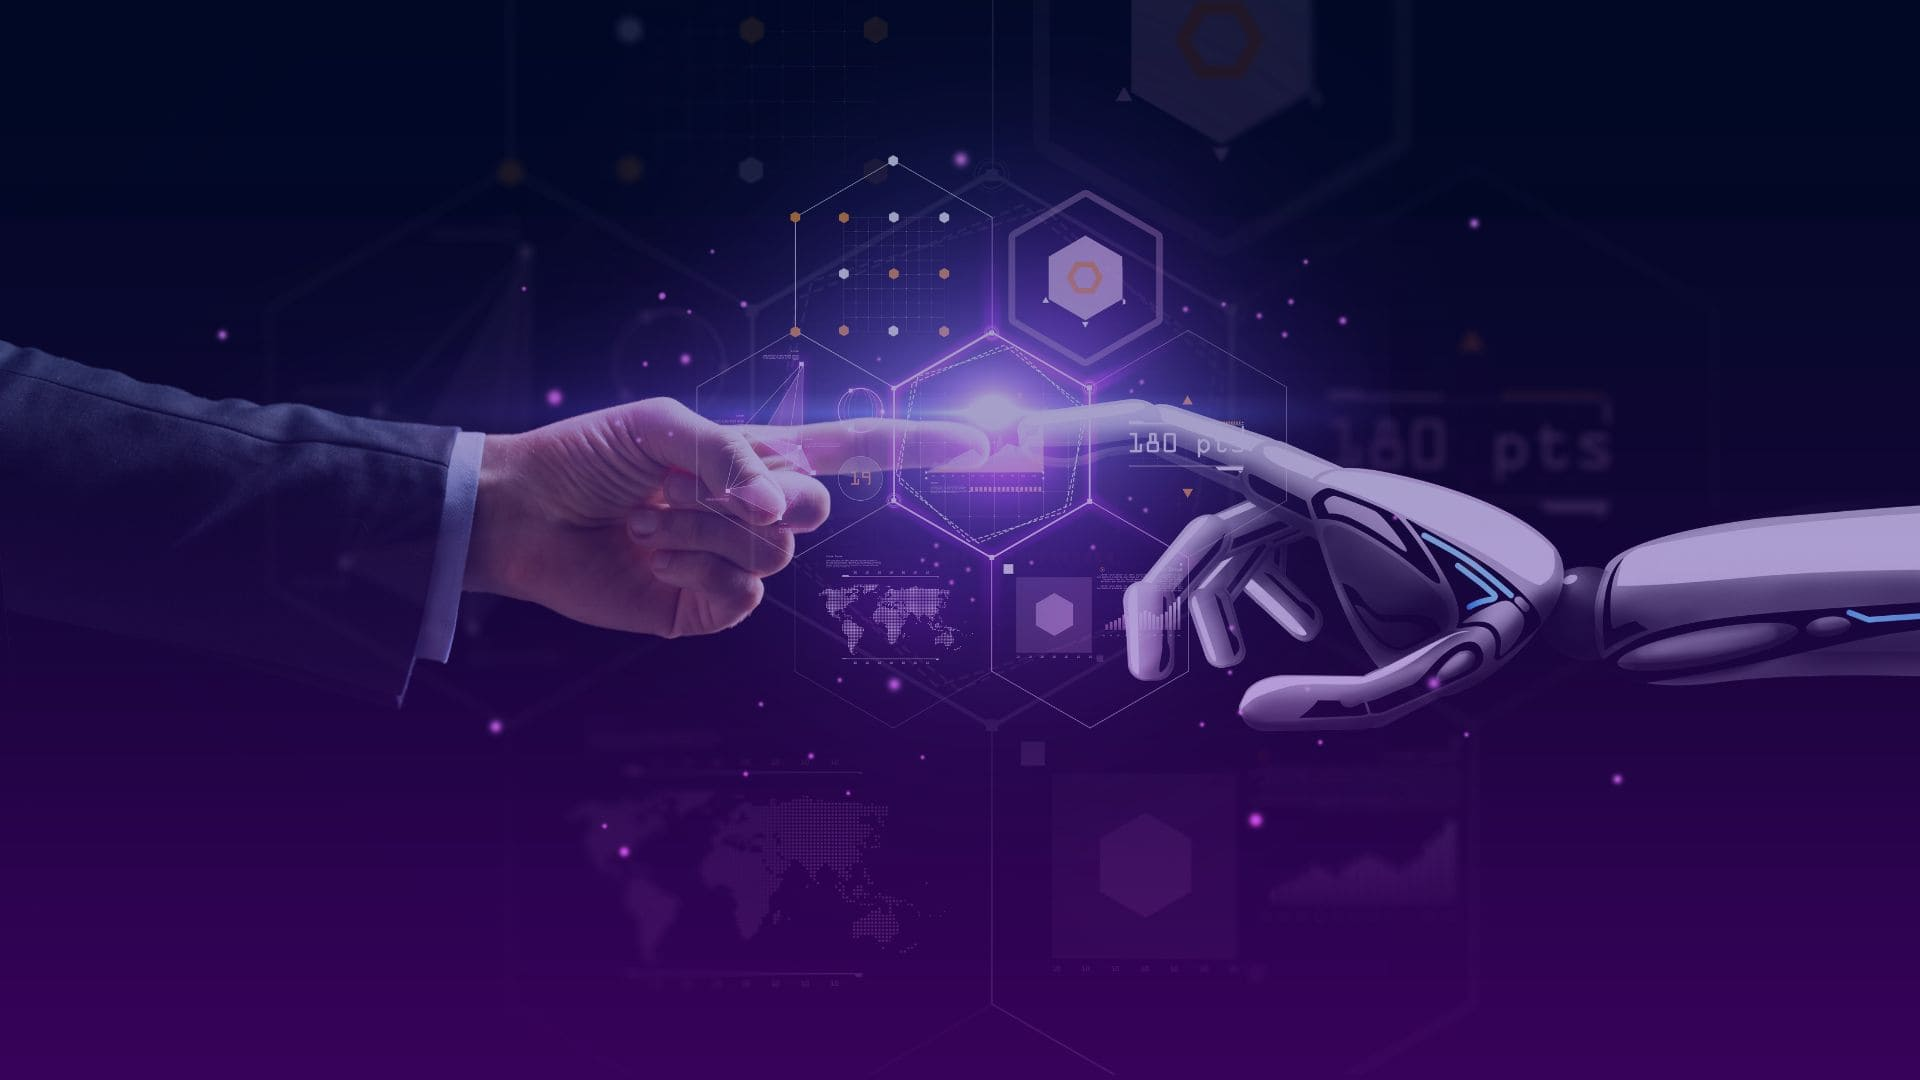
\includegraphics[width=\paperwidth,height=\paperheight]{images/capa.jpg}
}
	

\begin{frame}

\end{frame}
}


%% Titulo

{
\usebackgroundtemplate{
\centering

\includegraphics[width=\paperwidth,height=\paperheight]{images/fundo.pdf}
}
	
% Frame 3: plano de fundo
\begin{frame}
\maketitle
	
\end{frame}
}

{
\usebackgroundtemplate{
\centering

\includegraphics[width=\paperwidth,height=\paperheight]{images/fundo.pdf}
}

\begin{frame}
	\centering
	\frametitle{\textcolor{blue}{Sumário}}
    %\large
	\setbeamercolor{section in toc}{fg=blue,bg=blue}
    \tableofcontents[currentsection,sectionstyle=show/shaded,subsectionstyle=show/show/shaded]
\end{frame}

}








\section{Introdu\c{c}ão} 

\section{Inteligência versus aprendizado}

\section{Trazendo o aprendizado para um computador}

\section{Conceitos envolvidos}

\section{O Perceptron e as demais RNAs}

\section{Mãos à obra}

\section{Um exemplo prático}
{
\usebackgroundtemplate{
\centering
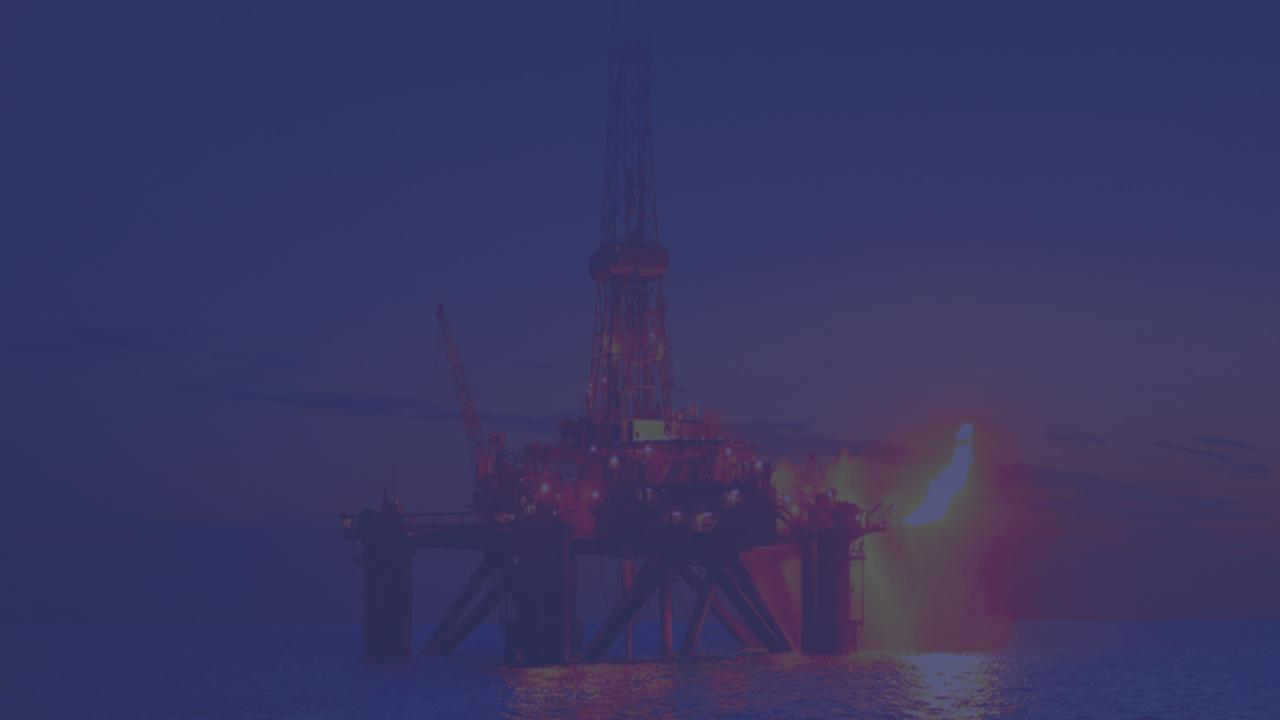
\includegraphics[width=\paperwidth,height=\paperheight]{images/fundonovo.jpg}
}
\begin{frame}
\vspace{2cm}
\begin{center}
\huge
	\textcolor{orange}{Um exemplo prático}
\end{center}

\end{frame} 
}


\section{Bate-papo}



















%%%%%%%%%%%%%%%%%%%%%%%%%%%%%%%%%%%%%%% REFERENCES %%%%%%%%%%%%%%%%%%%%%%%%%%%%%%%%%%%%%%%%%%%%%%%%%


{
\usebackgroundtemplate{
\centering

\includegraphics[width=\paperwidth,height=\paperheight]{images/fundo.pdf}
}
\begin{frame}[allowframebreaks]
\frametitle{Referências}
%\beamertemplatetextbibitems
\tiny
%\bibliographystyle{apalike}
%\bibliography{references}

\end{frame}



\end{document}
